% Some LaTeX commands I define for my own nomenclature.
% If you have to, it's better to change nomenclature once here than in a 
% million places throughout your thesis!



%======================================================================
\chapter{Methodology }
%======================================================================

\section{Methodology for achieving Objective - 1 }

\textbf{Objective 1: To understand foreign visitors' attitudes toward Safety Tips.}

For research objective 1, the nationality data in item 1 and item 6 were used, containing two tasks. While considering that the main users of Safety Tips are foreign visitors, only the sample of foreign respondents was selected for this part of the analysis, and the sample of Japanese respondents was excluded in this part. So the total number of samples was 1500.

The first task is to summarize the questionnaire's results from Q15 to Q17. The findings will show the popularity among foreign visitors, past usage experience of foreign respondents, and foreign respondents' attitude toward Safety Tips in each country, as well as the differences among respondents from the following five countries which are China, South Korea, Indonesia, Thailand, and the UK.

The second task was based on the answers to Q15 and Q16. As Q15 was 'do you know Safety tips or not?', and Q16 was 'Did you use safety tips before or not?', these two questions can clarify respondents' past usage of Safety Tips. The answers to Q15 had three options: Know exactly, Heard safety tips before, and Do not know. If the respondent answered 'Know exactly' or 'Heard Safety tips before', the respondent will continue to answer Q16, if the respondent answers 'Do not know', the respondent will directly skip to Q17. The answers to Q16 are 'used Safety tips before.' and 'never used it before. Therefore, based on the answers to these two questions, all respondents were divided into the following five groups: 'Know exactly and used Safety tips before', 'Know exactly but never used Safety tips before. before', 'Heard Safety tips before and used it before, 'Heard Safety tips before but never used it before, and 'Do not know and never used before. The sample sizes for each group are shown in Figure~\ref{fig6}, which are 'Know exactly and used Safety tips before': 357; 'Know exactly but never used Safety tips before': 90; 'Heard Safety tips before and used it before: 134; 'Heard Safety tips before but never used it before': 465 people; 'Do not know and never used before': 454 people. The results will show whether the two factors of respondents' past awareness and whether they used it before had an impact on their attitudes toward Safety Tips.


%%%%%%%%%%%%%%%%%%%%%%%
%\iffalse
\begin{figure*}[h]
  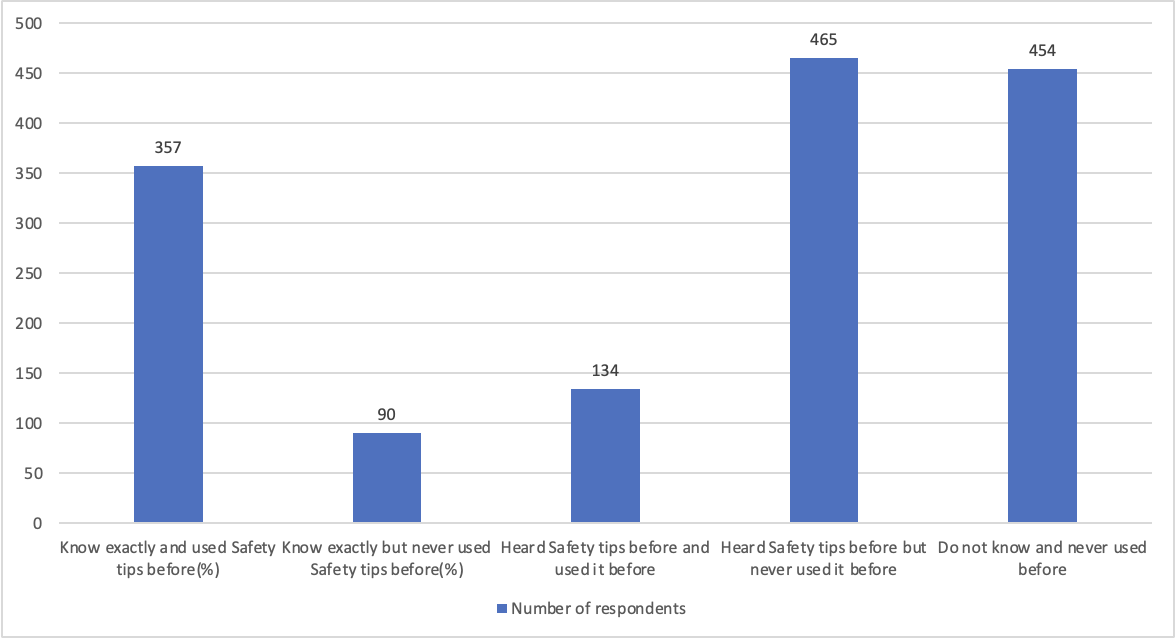
\includegraphics[width=\linewidth]{Figure/Figure6.jpg}
  \centering
  \caption{Number of respondents in each group. }
  \label{fig6}
\end{figure*}
%\fi




\section{Methodology for achieving Objective - 2 }
\textbf{Objective 2: To explore how respondents' attitudes toward Safety Tips are influenced by their characteristics. }

For research purpose 2, the data of Item 1, Item 2-4, and Item 6 were used. This part will continue to look into the impact of foreign respondents' personality characteristics on their attitude toward Safety Tips. As this part continues to focus on foreign visitors, and considering the attitudes of the respondents who have used this application about Safety Tips is even more telling, so for the Structural Equation Modeling, we only selected the sample data that give 'used before' answer in Q16. Therefore, the data sample amount is 491. Based on the discussion of sample size, the following suggestions for minimum sample sizes are offered based on the model complexity and basic measurement model characteristics~\cite{ref15}:

\begin{itemize}
\item Minimum sample size--100: Models containing five or fewer constructs, each with more than three items (observed variables) and with high item communality (.6 or higher).
\item Minimum sample size-150: Models with seven constructs or less, modest communalities(.5), and no under-identified constructs.
\item Minimum sample size-300: Models with seven or fewer constructs, lower communality(below .45), and/or multiple under-identified (fewer than three) constructs.
\item Minimum sample size-500: Models with large numbers of constructs, some with lower communality, and/or having fewer than three measured items.
\end{itemize}
The current sample data amount is available in this study. 

\textbf{Structural Equation Modeling.} Structural Equation Modeling will be used to analyze this part. Structural Equation Modeling is a statistical method based on Regression Models for Latent Variables, and SEM is a multiple regression model that allows us to test the theoretical model by testing the hypothesis to better understand the variables in our hypothesis with a clearer causal relationship between them~\cite{ref13}. Structural Equation Modeling can consider and deal with multiple dependent variables at the same time and allow for measurement error in both independent and dependent variables. Also, Structural Equation Modeling can estimate both factor structure and factor relationships, which could be more useful for this research. In summary, the variables used in SEM include unobservable latent variables and observable indicator variables. Latent variables can usually be measured by several indicator variables~\cite{ref14}. Therefore, this study will use Structural Equation Modeling to explore whether factors will have an impact on respondents' attitudes toward Safety Tips or not. For the Implementation of Structural Equation Modeling, there are 9 steps as follows. 

\begin{itemize}
\item Constructing theoretical models
\item Formulate the research hypothesis
\item Define variables
\item Sample data collection and processing
\item Reliability and validity testing (EFA/CFA)
\item Model Fit Test
\item Model adjustment and modification
\item Path coefficient analysis
\item Hypothesis testing and conclusion analysis
\end{itemize}

\subsection{Step 1. Constructing theoretical models}
The first step in constructing a Structural Equation Modeling is to construct a theoretical model, identify the research topic, transfer the research problem into several academic concepts, and then construct the basic framework among the different concepts. For this study, the research topic was to explore what factors influence foreign visitors' attitudes toward Safety Tips. Therefore, the basic framework extracted from this is 'Attitude toward Safety Tips' and some related factors. From Table~\ref{table1} we can find that the survey questions are divided into items, and these divided items are the latent variables that we could use in Structural Equation Modeling. Item 1 is demographic information; Item 2 is disaster prevention consciousness; Item 3 is disaster response education, experience on earthquakes; Item 4 is knowledge and perception on earthquakes; Last item 6 is the perception on Safety Tips. Combining the questions in the online survey mentioned before, we initially formulated four latent variables using for constructing Structural Equation Modeling, which are Disaster Prevention Consciousness, Disaster Knowledge, Training experience, and Attitude toward Safety Tips. For some manifest variables, we need to first determine whether the differences in demographic factors are significantly different in the responses of 'Attitude toward Safety Tips' by independent-samples T-test and Analysis of variance (ANOVA). If the results show a significant difference, they can be placed as manifest variables in the SEM. If no significant differences were shown, there was no need to include them as manifest variables. The results of the Independent-samples T-test and ANOVA will be explained in Chapter~\ref{c5}. 


\subsection{Step 2. Formulate the research hypothesis}
The second step in constructing Structural Equation Modeling is to formulate the research hypothesis. Based on the theoretical framework, the path relationships need to extract meaningful latent variables to enrich the path relationships. To construct Structural Equation Modeling for this research, it is necessary to make hypotheses between Disaster Prevention Consciousness, Disaster Knowledge, Training experience, and Attitude toward Safety Tips based on previous research. 

\begin{itemize}
\item Individual characteristics (risk belief, connectedness, knowledge, and past experience with hurricanes), travel-related variables, and the socio-demographic characteristics of tourists influence their decision regarding whether or not to evacuate in the event of a hurricane.~\cite{Cahyanto2014AnEE}
\item The tourists' evacuations were also influenced by tourists' hurricane knowledge and past experience.~\cite{Cahyanto2016StatedPO}
\end{itemize}

Based on these two studies, we can construct a relationship that knowledge, travel-related variables, and socio-demographic characteristics could relate to Evacuation Behaviors, shown in Figure~\ref{fig7}.

%%%%%%%%%%%%%%%%%%%%%%%
%\iffalse
\begin{figure*}[h]
  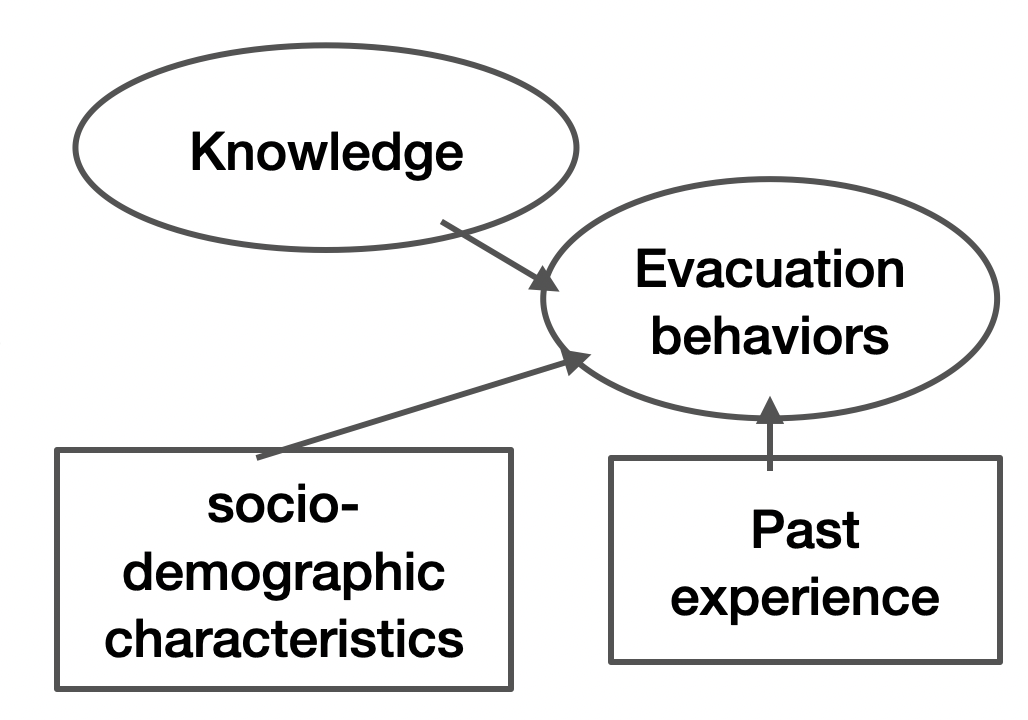
\includegraphics[width=0.5\linewidth]{Figure/Figure7.png}
  \centering
  \caption{Hypothesis base on previous research - 1 }
  \label{fig7}
\end{figure*}
%\fi

\begin{itemize}
\item Evacuation is significantly related to Socio-demographic factors, such as age, gender, etc, Socioeconomic factors, like educational attainment or household characteristics, etc, Personal characteristics, like hazard experience, knowledge, abilities/impairments, etc. Also, evacuees tend to make use of their familiarity with the surroundings based on their knowledge.~\cite{Wang2021IncorporatingHF}
\end{itemize}

Based on this study, we can construct a relationship that age, gender, hazard experience,  educational attainment, knowledge, abilities could relate to Evacuation Behaviors, shown in Figure~\ref{fig8}. 

\begin{figure*}[h]
  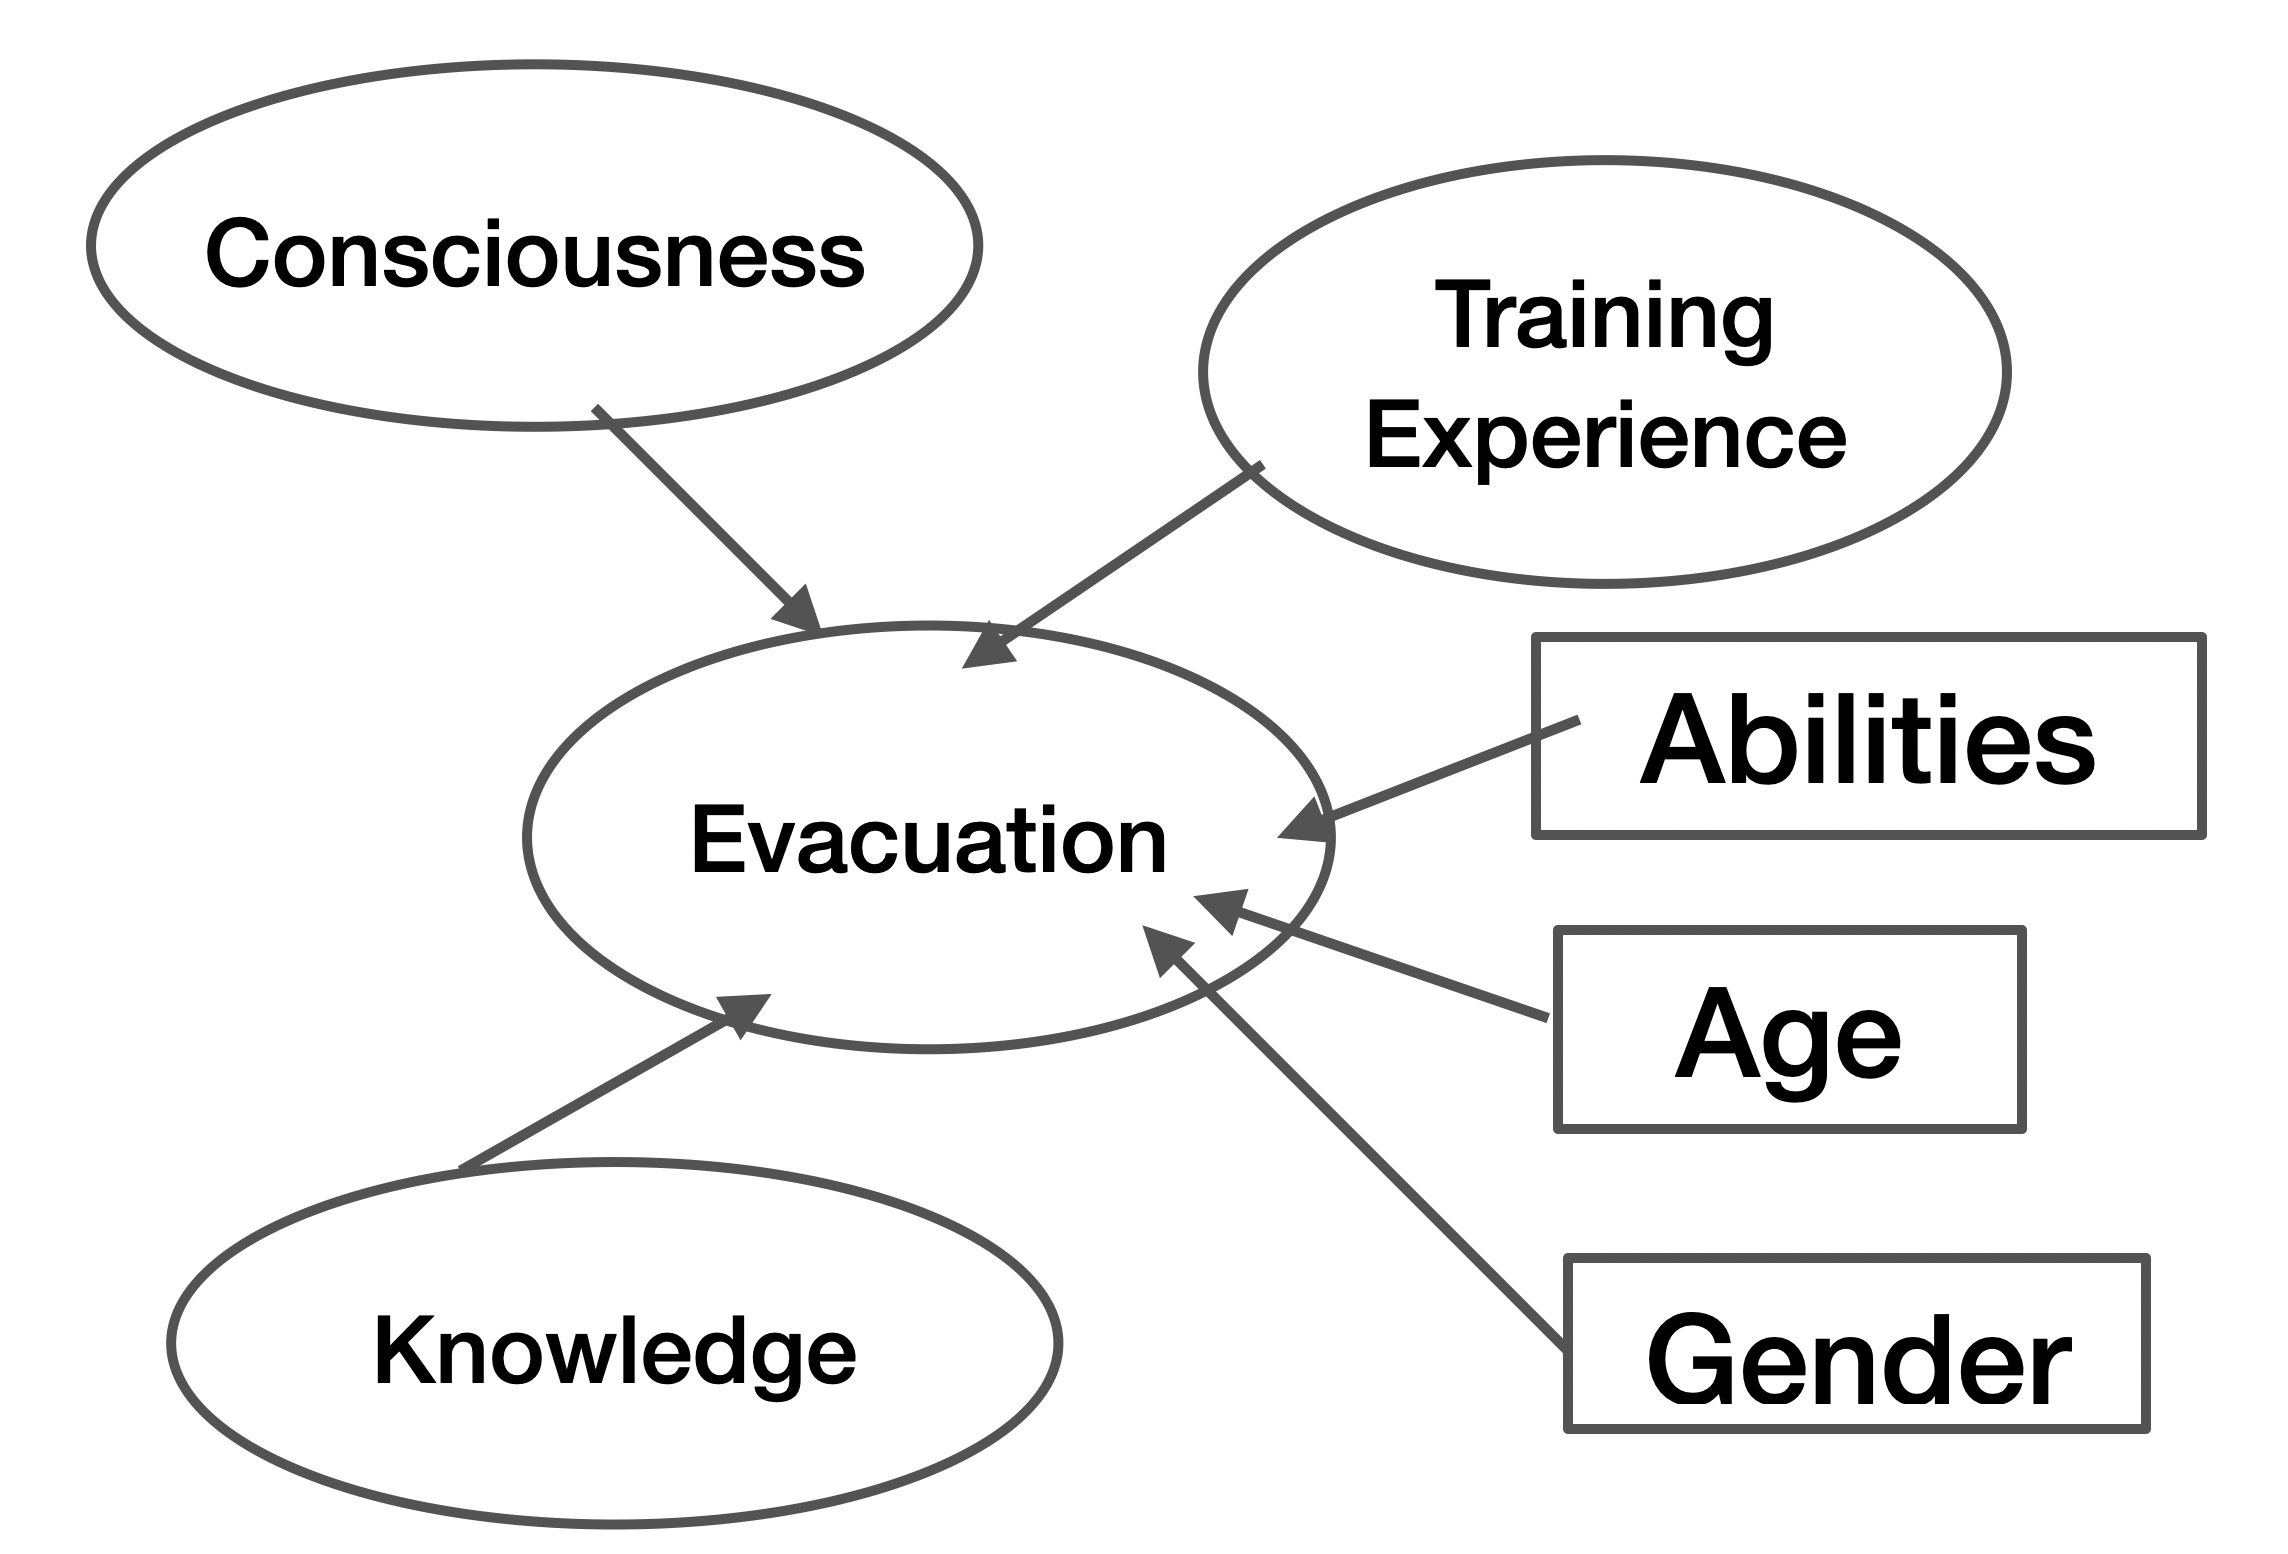
\includegraphics[width=0.5\linewidth]{Figure/Figure8.png}
  \centering
  \caption{Hypothesis base on previous research - 2 }
  \label{fig8}
\end{figure*}

In this study, we initially formulated three hypotheses (H1- H3 ) corresponding to the causal relationships between four latent variables based on the above results, which are shown in Figure~\ref{fig30}.

\begin{itemize}
\item[\textbf{H1}] Disaster Prevention Consciousness has a positive impact on Attitude toward Safety Tips.
\item[\textbf{H2}] Disaster Knowledge has a positive impact on Attitude toward Safety Tips.
\item[\textbf{H3}] Training Experience has a positive impact on Attitude toward Safety Tips.
\end{itemize}

%%%%%%%%%%%%%%%%%%%%%%%
%\iffalse
\begin{figure*}[h]
  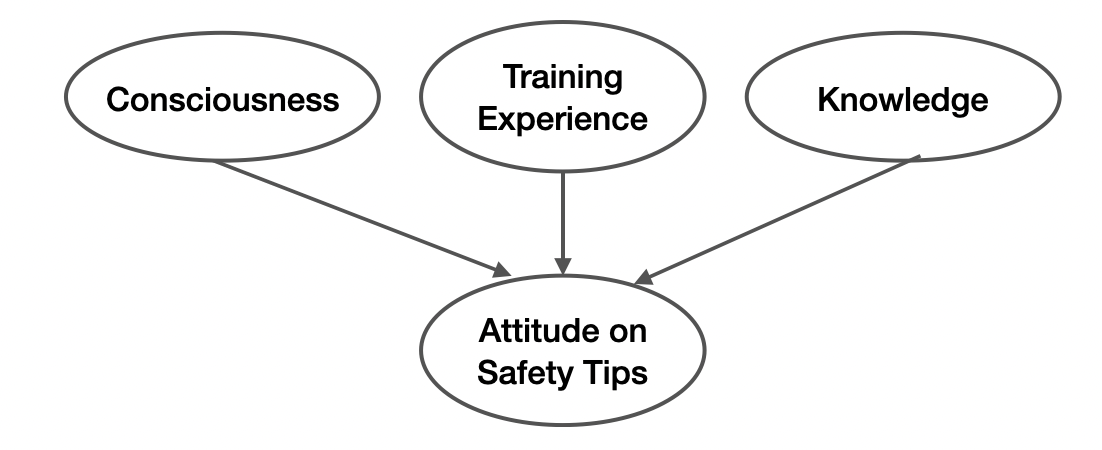
\includegraphics[width=0.5\linewidth]{Figure/Figure30.jpg}
  \centering
  \caption{Initial hypothesis used for SEM}
  \label{fig30}
\end{figure*}
%\fi

Each latent variable is represented by multiple indicators, and the summary statistics of these indicators are shown in Table~\ref{table5}. The latent variable 'Disaster Prevention Consciousness' has 5 manifest variables, which are disastrous imagination (Q1), sense of crisis (Q2), other-directed type (Q3), anxiety (Q4), apathy about disasters (Q5). The latent variable 'Disaster Knowledge' has 2 manifest variables, which are knowledge about earthquakes (Q9) and knowledge of how to respond to a disaster (Q10). The latent variable 'Training Experience' has 2 manifest variables, which are the total score of earthquake/tsunami/typhoon/fire training experiences. (Q6) and the number of times participating in earthquake/tsunami/typhoon/fire disaster training (Q7). Latent variable 'Attitude toward Safety Tips' has 4 manifest variables, which are trust level (Q17\_1), the priority of use (Q17\_2), usefulness (Q17\_3), and the possibility of future use (Q17\_4). In addition to this, there are some directly observable manifest variables, such as demographic variables, etc. These variables will be involved in the SEM as manifest variables. Since it is uncertain whether these variables affect their attitude towards Safety Tips, a sample test will be conducted subsequently. There are 6 manifest variables, which are Age (FQ3), Gender (FQ2), number of visits to Japan within 1 year (FQ5), number of visits to any country in the world within 1 year (FQ4), Japanese level (FQ7), and the severity of the earthquake experienced (Q8). Therefore, the final Structural Equation Modeling shows in Figure~\ref{fig9}.

%%%%%%%%%%%%%%%%%%
%\iffalse
\begin{table}[h]
  \caption{Latent variables and manifest variables used for SEM. }
  \label{table5}
  \centering
  \begin{tabular}{|c|l|c|}
  \hline
  Latent variables &  \multicolumn{1}{c|}{Manifest Variables} &  \begin{tabular}{c}Number of\\variables\\included \end{tabular} \\
  \hline
  \multirow{5}{*}{\begin{tabular}{c}Disaster prevention\\consciousness \end{tabular}} & Disastrous Imagination (Q1) & 1\\
  \cline{2-3}
        & Sense of crisis (Q2) & 1 \\
  \cline{2-3}
        & Other-directed type (Q3) & 1\\
  \cline{2-3}
        & Anxiety (Q4) & 1\\
  \cline{2-3}
        & Apathy about disasters (Q5) & 1\\
  \hline
  \multirow{2}{*}{Disaster knowledge} & Knowledge about earthquakes (Q9) & 1\\
  \cline{2-3}
        & Knowledge of how to respond to a disaster (Q10) & 1\\
  \hline
  \multirow{2}{*}{Training experiences} & \begin{tabular}{l}Total score of earthquake/tsunami/typhoon/\\fire training experiences. (Q6)\end{tabular} & 4 \\
  \cline{2-3}
        & \begin{tabular}{l}Number of times participating earthquake/\\tsunami/typhoon/fire disaster training (Q7)\end{tabular} & 4\\
  \hline
   \multirow{4}{*}{\begin{tabular}{c}Attitude toward\\Safety Tips\end{tabular}} & Trust level & 1 \\
  \cline{2-3}
                                            & Priority of use & 1\\
  \cline{2-3}
                                            & Usefulness & 1 \\
  \cline{2-3}
                                            & Possibility of future use & 1 \\
  \hline
   / & Age & 1\\
  \hline
   / & Gender & 1\\
   \hline
   / & Number of visit Japan within 1 year & 1\\
   \hline
   / & \begin{tabular}{l}Number of visit any country in the world\\within 1 year\end{tabular} & 1 \\
   \hline
   / & Japanese level & 1 \\ 
   \hline
   / & The severity of the earthquake experienced & 1 \\
   \hline
  \end{tabular}
\end{table}
%\fi
%%%%%%%%%%%%%%%%%%%%%%%%%%%%%%%%
%\iffalse


\begin{figure*}[h]
  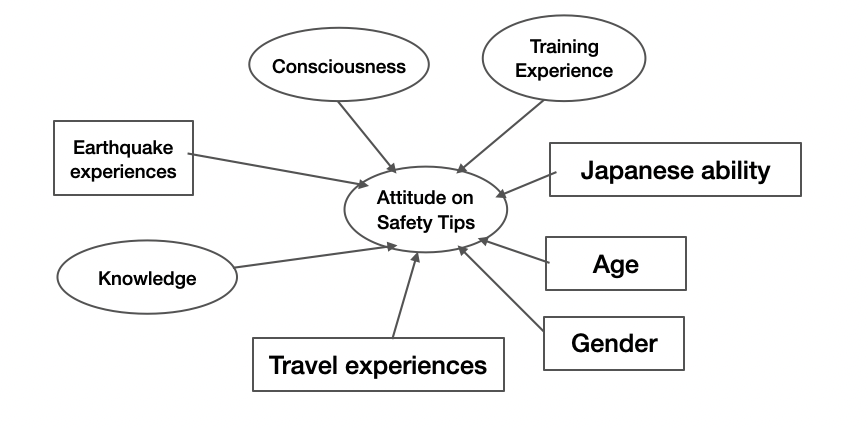
\includegraphics[width=\linewidth]{Figure/Figure9.png}
  \centering
  \caption{Final Hypothesis used for SEM }
  \label{fig9}
\end{figure*}


\subsection{Step 3. Define variables}
The third step is to define each variable. This part requires a definition of all the variables. The definitions of manifest variables are shown in Table~\ref{table2item2}, Table~\ref{table2item3}, Table~\ref{table2item4}, and Table~\ref{table2item6}, including Disaster Prevention Consciousness, Disaster Knowledge, Training experience, and Attitude toward Safety Tips. The definitions of manifest variables are shown in Table~\ref{table2item1} and  Table~\ref{table2item3}, including Age (FQ3), Gender (FQ2), number of visits to Japan within 1 year (FQ5), number of visits to any country in the world within 1 year (FQ4), Japanese level (FQ7), and the severity of the earthquake experienced (Q8).


\subsection{Step 4. Sample data collection and processing}
The data are offered by the Economic and Social Research Institute mentioned in Chapter~\ref{c3}, and the data processing methods are shown in the following. 

\begin{itemize}
\item Item 1 (FQ2-FQ5,FQ7)
\end{itemize}

FQ2: (Male) = 1; (Female) = 2;

FQ3: (Age\,Under\,15) = 1; (Age 16-19) = 2; (Age 20-29) = 3; (Age 30-39) = 4; (Age 40-49) = 5; (Age 50-59) = 6; (Age 60-69) = 7; (Age Over 70) = 8;

FQ4\&FQ5: (0 time) = 0; (1 time) = 1; (2 times) = 2; (3 to 4 times) = 3; (5 to 6 times) = 4; (7 to 9 times) = 5; (Over 10 times) =6;


FQ7: (Cannot understand) = 1; (Basic) = 2; (Intermediate) = 3; (Up Level) = 4; 

\begin{itemize}
\item Item 2 (Q1-Q5)
\end{itemize}

Since each of Q1-Q5 has four sub-problems. Here will use the mean values of the four sub-problems as the final data. For example, Q1 = $mean$ (Q1\_1, Q1\_2, Q1\_3, Q1\_4), Q2-Q5 are processed in the same way.

\begin{itemize}
\item Item 3 (Q6-Q8)
\end{itemize}

Q6 is about past disaster training participation experience. There are four types of disasters: Q6\_1 earthquake, Q6\_2 tsunami, Q6\_3 typhoon, and Q6\_4 fire. Each of them has 12 different types of training experience, shown as Q6\_1/2/3/4\_1 to Q6\_1/2/3/4\_12. Respondents answered with 'Yes' or 'No' in these questions. If none of them were experienced before, 'Yes' was selected in Q6\_1/2/3/4\_13 to indicate that the respondent did not have any of the 12 experiences mentioned above. 

Therefore, 

Q6\_1 = $sum$ (Q6\_1\_1 + Q6\_1\_2 +\dots+ Q6\_1\_12);

Q6\_2 = $sum$ (Q6\_2\_1 + Q6\_2\_2 +\dots+ Q6\_2\_12);

Q6\_3 = $sum$ (Q6\_3\_1 + Q6\_3\_2 +\dots+ Q6\_3\_12);

Q6\_4 = $sum$ (Q6\_4\_1 + Q6\_4\_2 +\dots+ Q6\_4\_12).

Q7 is times of past disaster training experiences. There are also four types of disasters: Q7\_1 earthquake, Q7\_2 tsunami, Q7\_3 typhoon, and Q7\_4 fire.
 
(one time) = 1; (2-3 times) = 2; (4-6 times) = 3; (Over 7 times) =4;

Q8 is about the severity of the earthquake experienced.

(MMI intensity 5 or less / intensity 3 or less) = 1; (MMI intensity 6 / intensity 4) = 2; (MMI intensity 7 / intensity 5 weak) = 3; (MMI intensity 8 / intensity 5 strong) = 4; (MMI intensity 9 / intensity 6 weak) = 5; (MMI intensity 10 / intensity 6 strong) = 6; (MMI intensity 11 to 12 / intensity 7) = 7; (no experience) = 8.


\begin{itemize}
\item Item 4 (Q9-Q10)
\end{itemize}

Q9 has six sub-problems, Q10 has nine sub-problems. Here will use the mean values of the sub-problems as the final data. 

Therefore, 

Q9 = $mean$ (Q9\_1, Q9\_2, \dots, Q9\_6);

Q10 = $mean$ (Q10\_1, Q10\_2, \dots, Q10\_9).

\begin{itemize}
\item Item 6 (Q15-Q17)
\end{itemize}

Q15: (Don't know) = 1; (Only heard name before) = 2; (Know exactly) = 3;

Q16: (Never used before) = 0; (Used before) = 1;
 
Q17\_1, Q17\_2, Q17\_3, Q17\_4: use original data.

\subsection{Step 5. Reliability and validity testing (EFA/CFA)}

The first measurement theory that we need to understand in Structural Equation Modeling is that the observed values equal true values plus bias and noise. Reliability means the degree to which the results are consistent when the same method is used to measure the same object repeatedly. As a result, Reliability indicates how much the measure is free from random error (noise). Reliability is the consistency, stability, and reliability of test results, and is generally expressed in terms of the internal consistency of the test. The higher the reliability coefficient, the more consistent, stable, and reliable the test results are. In addition, the systematic error has little effect on reliability in Reliability tests. Because systematic errors always affect the measurement values, in the same way, they do not cause inconsistency. On the contrary, random errors may cause inconsistency and thus reduce the difficulty. Reliability will be tested through the evaluation of Cronbach's alpha value by SPSS. 

Validity refers to the degree to which a measurement tool or instrument can accurately measure what is to be measured. As a result, Validity indicates how much the measure is free from systematic error (bias). Validity means that the results measured reflect what is intended to be measured and that the results measured are what was intended to be measured. Validity is an indicator of the degree of validity of a measurement instrument, i.e., the degree to which the instrument can measure the characteristics to be measured, and can be simply interpreted as the accuracy and usefulness of a test. 

There are two types of Validity Analysis, one is Exploratory Factor Analysis (EFA), which is generally used in SPSS. EFA is measured through dimensionality reduction. For example, if the questionnaire has 100 questions, then how many dimensions these 100 questions should be grouped into can be achieved by EFA. But most self-designed questionnaires, in fact, when designing the questionnaire, there is already a potential dimensional division. The other one is Confirmatory Factor Analysis (CFA). Compared with EFA, CFA can be used to check the compliance of the three types of validity, including the compliance of the model fit, the consistency of the indicators within each dimension, and the differentiation of the indicators from external indicators. CFA estimates latent variables based on correlated changes in the dataset, which can reduce data dimensionality, standardize the size of multiple metrics, and account for correlations inherent in the dataset~\cite{ref16}. CFA is generally used by Amos, and it is measured by Construct Validity, Convergent Validity, and Discriminant Validity. The main purpose of Construct Validity is to check the fitness of the whole model. If the fit is low, the model, the latent variables, and the relationships between the latent variables are adjusted to improve the fit. The adjustments are explained in subsection~\ref{s7}. 

The Convergent Validity looks at the strength of the correlation between several topics within the same dimension. 
Regarding Convergent Validity, it is used to assess the internal consistency of several items and has similarity with Cronbach's alpha. However, when there are multiple dimensions of the scale, it is not appropriate to use Cronbach's alpha to calculate its internal consistency reliability~\cite{ref29,ref30}. Convergent Validity is generally assessed using Composite Reliability (CR) and Average of Variance Extracted (AVE) to assess Convergent Validity. Convergent Validity~\cite{ref33} is estimated by the standardized factor loading and the respective error variance, the equation shown in the following Formula~\ref{for2}. $\lambda$ denotes the standardized factor loading for item $i$ and $\epsilon$ denotes the respective error variance for item $i$. The error variance is estimated based on the value of the standardized loading ($\lambda$) as Formula~\ref{for3}. And the R-square value is the percent of the variance, which is explained by the latent variable. It is estimated based on the value of the standardized loading ($\lambda$) as Formula~\ref{for4}. In this study, we will calculate CR value by Composite Reliability Calculator~\footnote{https://www.thestatisticalmind.com/composite-reliability/}. Higher CR indicates higher internal consistency and convergence of the conformation. The commonly used evaluation criterion in research is the one mentioned in the book Multivariate data analysis. 5th Edition~\cite{ref32}, that is CR value above 0.7 is acceptable. However, Fornell and Larcker (1981)~\cite{ref31} also suggested that a CR value above 0.6 is acceptable. 

\begin{equation}
\label{for2}
CR=\frac{(\sum \lambda_i )^2}{(\sum \lambda_i )^2+(\sum \epsilon _i )}
\end{equation}

\begin{equation}
\label{for3}
\epsilon_i = 1-\lambda_i^2  
\end{equation}

\begin{equation}
\label{for4}
r^2 = \lambda_i^2 = 1- \epsilon_i  
\end{equation}

Regarding AVE, AVE refers to the average of the explanatory power of the latent variables on the observed variables, and the equation is shown in the following Formula~\ref{for5}~\footnote{https://en.wikipedia.org/wiki/Average\_variance\_extracted}. Here, $k$ is the number of items, $\lambda_i$ is the factor loading of item $i$, and the $Var(e_i)$ is the variance of the error of item $i$. The higher the AVE, the higher the Convergent Validity. According to Fornell and Larcker (1981)~\cite{ref31}, the AVE value needs to be greater than 0.5. Squared Multiple Correlation (SMC) and Std. Factor Loading is used in the calculation of CR and AVE. A higher SMC indicates a higher proportion of true scores and can be used to calculate the confidence level.

\begin{equation}
\label{for5}
AVE = \frac{\sum_{i=1}^{k} \lambda_i^2 }{\sum_{i=1}^{k} \lambda_i^2+\sum_{i=1}^{k} Var(e_i)}
\end{equation}

Convergent Validity and Discriminant Validity can be viewed relatively. The Discriminant Validity is to see whether the differentiation between different dimensions and between topics meets the standard. There are three ways to achieve Discriminant Validity in CFA. The first is to compare the correlation coefficients of the two latent variables, and if their 95\% confidence intervals cover 1.00, it indicates that the constructs lack discriminant power. The second one is to compare two CFA models, one model is a validity model, and the other sets the correlation coefficient of the two potential variables to 1. That is, the fully correlated model/single-factor model. Theoretically, the latter will have a lower fit. If the former is significantly better than the latter, the discriminative power of the area between the two constructs is qualified. If the former is not significantly better than the latter, it means that the two constructs lack zone discrimination~\cite{ref34,ref35}. The third comparison was made using AVE to compare whether the mean AVE of two latent variables was greater than the squared correlation coefficient of the two latent variables~\cite{ref31}. The third method was adopted in this study. Because the questionnaire used in this study has a clear division of dimensions, EFA is not required for this study, and the results of Reliability Analysis and CFA will be presented in Chapter~\ref{c5}.


\subsection{Step 6. Model Fit Test}
Model Fit Test is primarily used for the CFA's Construct Validity test. The fit indices of the single-path coefficient test, which are the p-values and standard errors, and the overall model fit, which are the $\chi^2$ and RMSEA values, are used to evaluate the SEM~\cite{ref16}.

\begin{itemize}
\item \textbf{Chi-square Test ($\chi^2$):} It investigates the possibility of a discrepancy between the model-implied covariance matrix and the original covariance matrix. As a result, the non-significant difference is preferred. The Chi-square test should not be taken too seriously~\cite{ref22,ref23,ref24}, because it is very sensitive to sample size and is not comparable across different SEMs.
\item \textbf{Root Mean Square Error of Approximation (RMSEA):} RMSEA indicates 'badness of fit'. The RMSEA value of 0 means perfect fit, a higher value means short of fit~\cite{ref25}. RMSEA could be less sensitive to sample size than the Chi-square test, so RMSEA can be more useful when detecting model misspecification.
\item \textbf{Comparative Fit Index (CFI):} The amount of variance accounted for in a covariance matrix is represented by the CFI. Its value ranges from 0.0 to 1.0. A higher CFI value indicates a more accurate model fit. Compared with the Chi-square test, CFI can be less sensitive to sample size~\cite{ref26}.
\end{itemize}

In general, the more fit indices that are applied to SEM, the more likely it is that a misspecified model will be rejected, and the less likely it is that a good model will be rejected. As a result, the study must employ at least two distinct fit indices~\cite{ref17}. Some indices have recommended cutoff values, but no indices can be utilized as the standard for all applications~\cite{ref18,ref19,ref20,ref21}. Fan (2016)~\cite{ref16} mentioned other types of evaluation values for model fit, but this study decided to use the common evaluation values that were detailed mentioned above. 

\subsection{Step 7. Model adjustment and modification}
\label{s7}
Based on the structural validity results discussed earlier, the next step is to revise and adjust the Structural Equation Modeling. Therefore, the core of model revision and adjustment is to revise and optimize the measurement model for each latent variable to ensure that the overall model fitness is up to standard. The method of optimizing the measurement model, in addition to removing the less significant variables through the reliability results of SPSS, is to modify the indicator correction suggestions through the output of Amos. In general, there are two indicators. The first one is the Standardized Regression Weights (SRW), or Squared Multiple Correlation (SMC), which is the square of the SRW, and the SRW should be greater than 0.7 and the SMC should be greater than 0.5~\cite{ref15,ref27}. Another one is the Modification Indices. By M.I. value of covariances in the modification indices results. M.I. value refers to the amount of change that can be reduced by the corrected chi-square value, and the higher the value, the more it helps to correct the model. However, because the correlation between residuals is not academically interpretable. This is because the premise assumptions state that the residuals are independent. Therefore, correcting the model is done by removing the problem itself where the residuals have the greatest impact. As mentioned before, since the survey used in this study has a clear dimensional division, EFA was not performed. Therefore, this part of the model fitness adjustment will be performed with the first method as the main one.


\subsection{Step 8. Path coefficient analysis}
First look at Unstandardized Estimates, which describes how many units the dependent variable increases for each unit increase in the independent variable. Before evaluating the SEM fit, the estimated coefficients must be checked by Offending estimates to determine whether they are outside the acceptable range. Specifically, the first should look at the estimated coefficients of the error terms, which should not be negative. Secondly, we have to look at the factor loadings and whether the path coefficients are significant. Next, we look at the Standardized Estimates, which describes how many standard deviations the dependent variable will increase for each standard deviation increase in the independent variable. The factor loading of the measurement model should be greater than 0.7 and the SMC greater than 0.5, which proves to be very good; However, in general, the factor loading of the scales developed by social science researchers is not too high considering that it may be limited by the nature of the measurement (e.g., the range of attitude measurement is too wide and not easily focused, the construct is too vague and not easily defined), the external interference and measurement error, or even the nature of the construct. Tabachnica and Fidell, (2007)~\cite{ref28} suggest that a factor loading of 0.55 or higher and an SMC of 0.3 or higher can be declared good. As for the structural model of SMC, the main focus on significance is sufficient. To summarize, Unstandardized Estimates are used to see if they are significant, and Standardized Estimates are used to see the magnitude of the influence factors.


\subsection{Step 9. Hypothesis testing and conclusion analysis}
The hypothesis testing and conclusion analysis section is equivalent to a summary of SEM. We need to describe in detail the SEM model, the results of the model fitness, and the significance of the hypothesis relationships. The results are used to summarize the similarities/differences between the original hypothesis of the study and the results given by SEM, and to give an analysis based on the results. Finally, it is considered that this study needs to propose some suggestions for the future development of Safety Tips, so a proposal will be presented based on the conclusions presented in the results.





\section{Methodology for achieving Objective - 3}

\textbf{Objective 3: To explore patterns of information seeking and evacuation behaviors.}

For research objective 3, this study wanted to explore respondents' information-seeking behaviors and evacuation behaviors through their selections of behaviors. In order to understand which of the behaviors are preferred and which are selected more frequently, we chose to measure both the selected rate and the selected score. The calculation of the selected rate and the selected score will both do three times, for 300 Japanese samples, 1500 foreign visitors samples, and 1800 of all respondents' samples.

\subsection{Selected Rate}
Because the selected rate wants to explore which behaviors are used more, this part does not take the order factor into account. No matter the behavior is selected in which order, it will count as 1 point. The selected rate is equal to the Sum selected point divided by the sample number, shown in Figure~\ref{fig10}.

%%%%%%%%%%%%%%%%%%%%%%%%%%%%
%\iffalse
\begin{figure*}[h]
  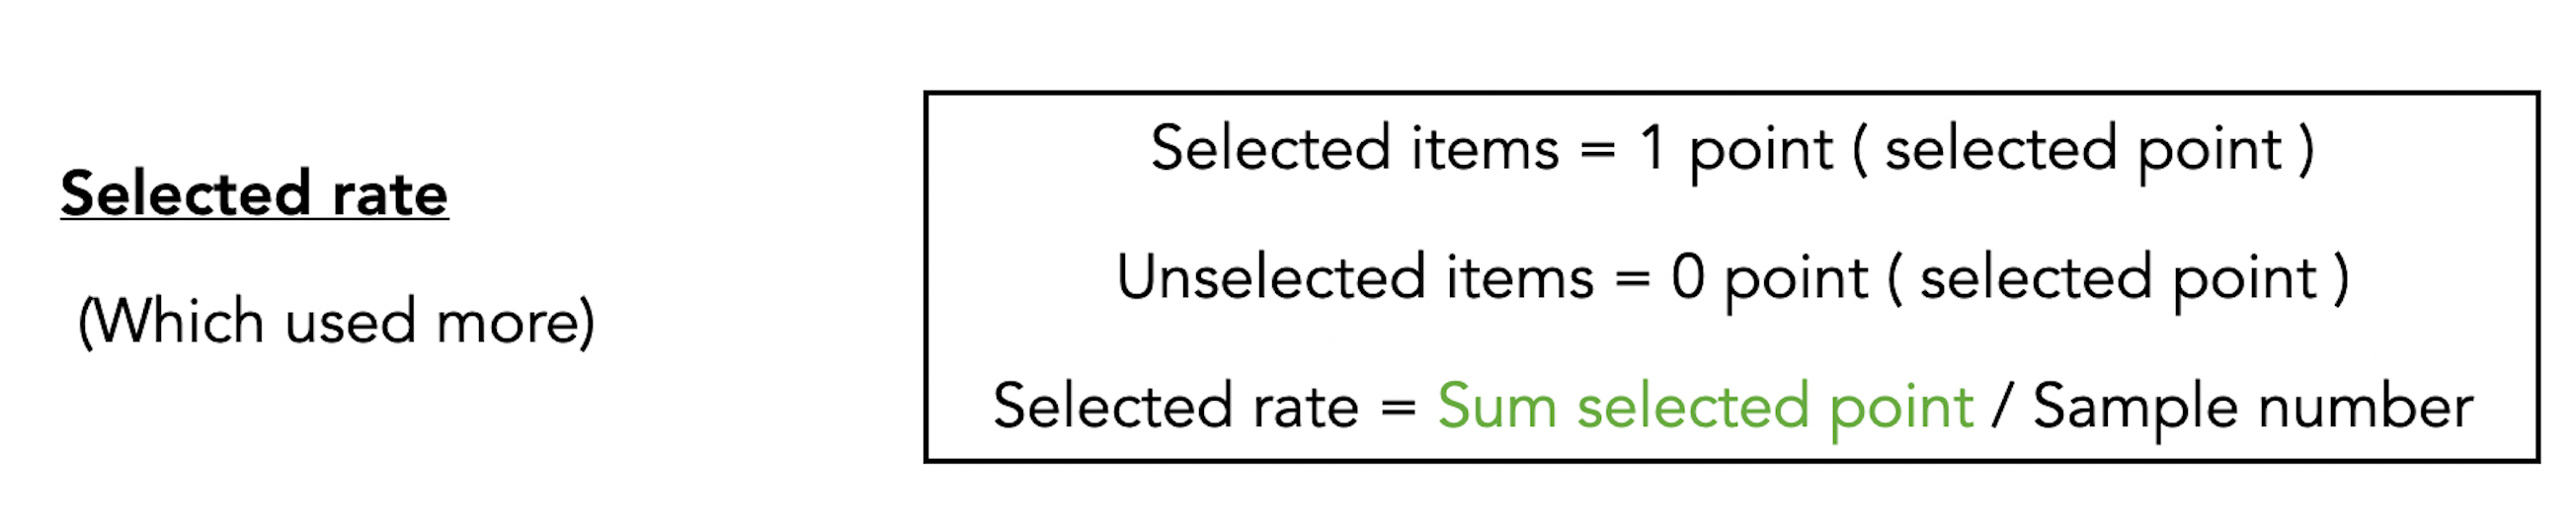
\includegraphics[width=\linewidth]{Figure/Figure10.png}
  \centering
  \caption{Selected rate }
  \label{fig10}
\end{figure*}
%\fi

\subsection{Selected Score}

Since the Selected score wants to explore which behaviors are used first, this part needs to take the order factor into account. The higher the preference is, the higher the score will be. So the first selected action is scored as 5, the second is scored as 4, the third is scored as 3, the fourth is scored as 2, and the last selected action is scored as 1. The Selected score is equal to the total score divided by the Sum selected point, shown in Figure~\ref{fig11}.

%%%%%%%%%%%%%%%%%%%%%%%%%%%
%\iffalse
\begin{figure*}[h]
  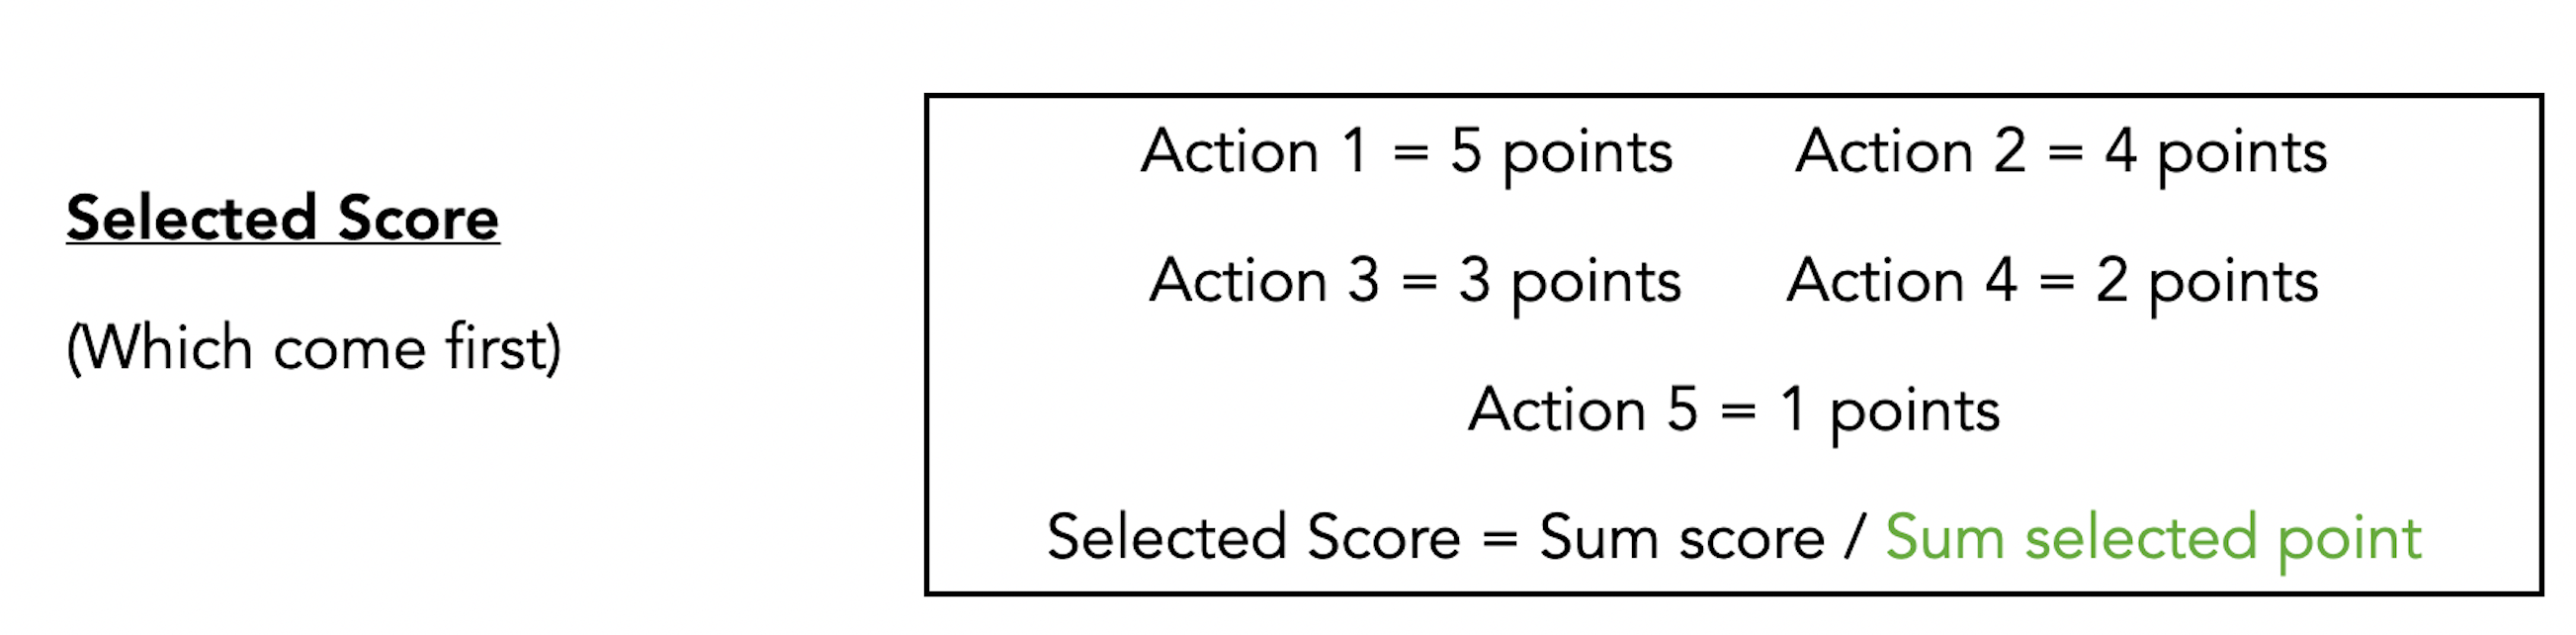
\includegraphics[width=\linewidth]{Figure/Figure11.png}
  \centering
  \caption{Selected score}
  \label{fig11}
\end{figure*}
%\fi

\subsection{Behavior Pattern}

In the analysis of the selected score and selected rate of study objective 3, we will find that all the results will be relatively scattered. This is because, in this study, the number of available selections is relatively large, which makes the results more scattered. However, from the results, we can see that there could be similarities in the behavior patterns of people. Here the word 'pattern' means behavior patterns, not specific behavior. For example, the behavior of  'collecting information' is the same, the difference is how to collect information, from official websites, from disaster prevention software, from disaster prevention websites, from SNS, etc. So how to divide detailed behaviors into patterns? From the available selection, we can find that the behavior is mainly divided into two kinds, which are information-seeking behavior and evacuation behavior. First, regarding information-seeking behavior, we can find that there are two main patterns, one is 'No-face-to-face information seeking' and the other is 'Face-to-face information seeking'. And for the evacuation behavior, we can also find two main patterns, one is ' Self-evacuation behaviors ' and the other is ' Following evacuation guidance behavior '. Then, we divided all the selections into the patterns they belong to, which can be found in Figure~\ref{fig12}.

%%%%%%%%%%%%%%%%%%%%%%%%%%%
%\iffalse
\begin{figure*}[h]
  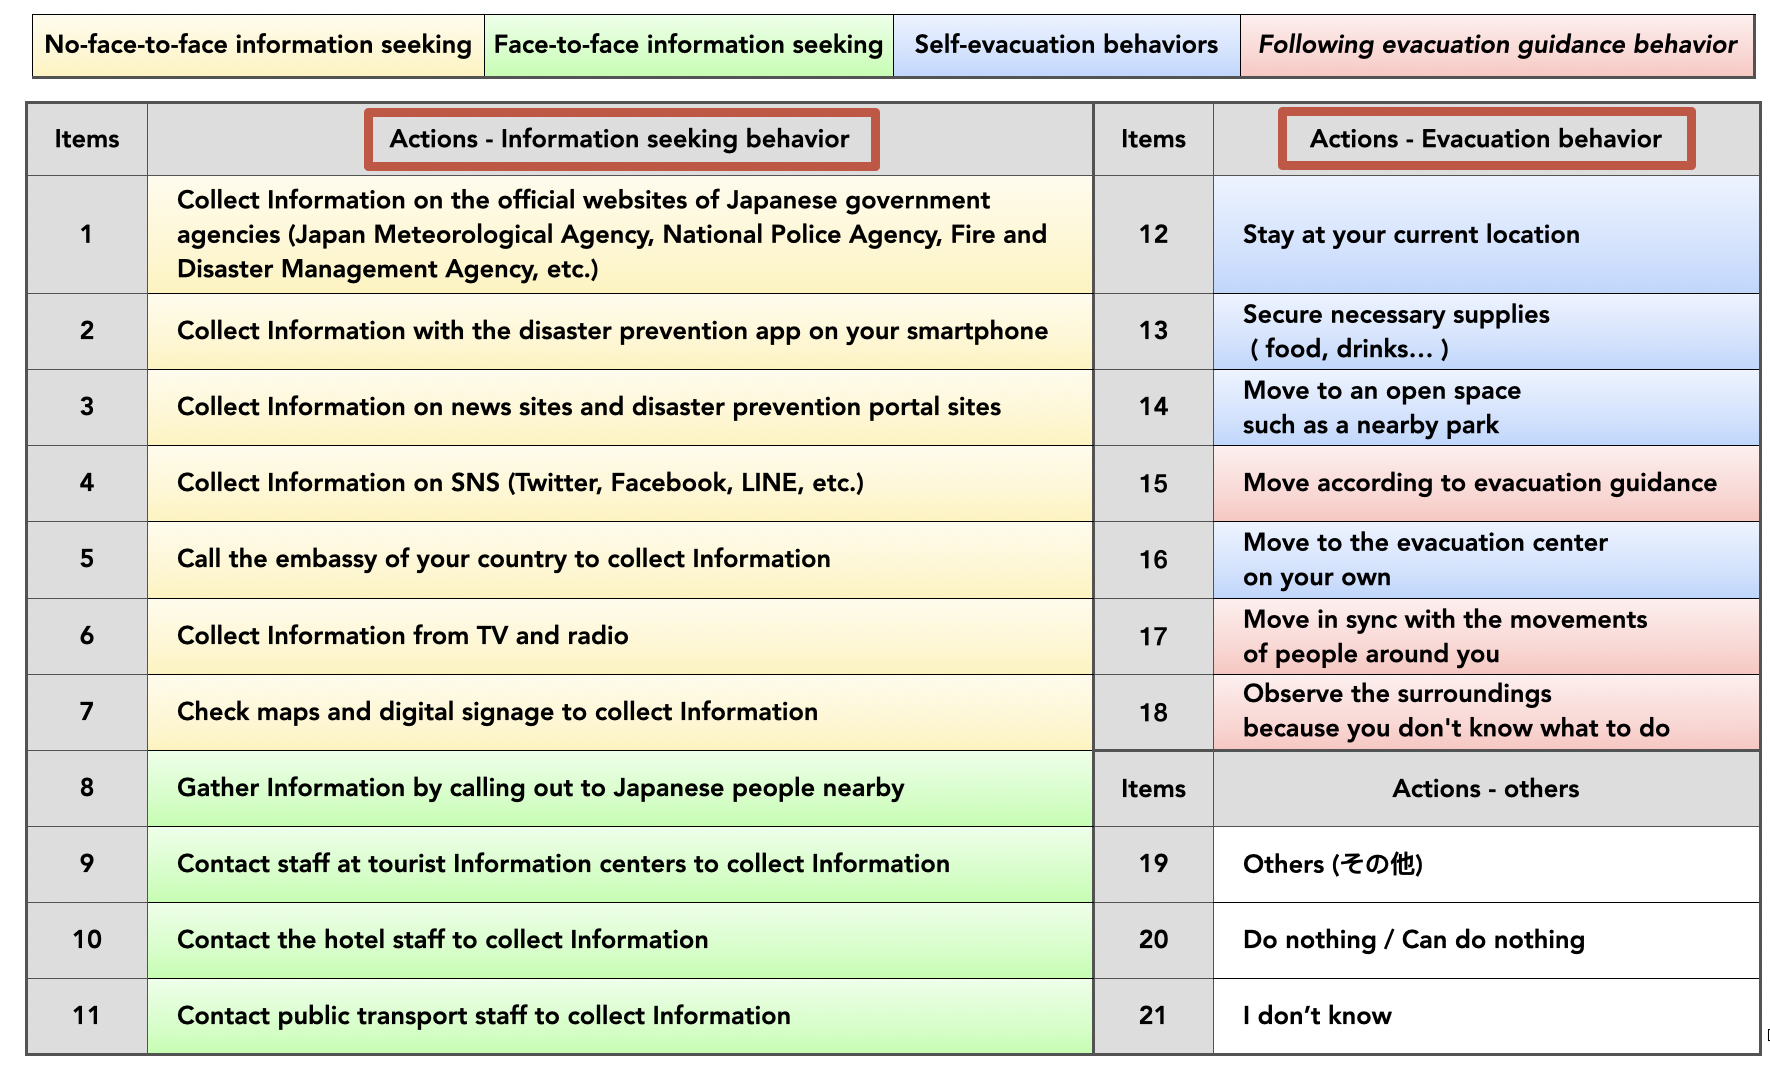
\includegraphics[width=\linewidth]{Figure/Figure12.png}
  \centering
  \caption{behavior patterns}
  \label{fig12}
\end{figure*}
%\fi

After attributing all the actions to the 4 patterns, we went through the flow of the respondents' actions with the help of the Sankey diagram. The Sankey diagram is a flow chart that shows the flow from each set of values to another set of values. The thickness of the lines expresses the number of values present in the group. In the Sankey diagram, the number indicates the No. of action, so 1-5 means the first action to the fifth action. Capital letters indicate behavior patterns.' No-face-to-face information seeking' is A; 'Face-to-face information seeking' is B; 'Self-evacuation behaviors' is C; 'Following evacuation guidance behavior' is D. Thus, the behavior from the first to the fifth cohort can be clearly represented in the results of the Sankey diagram. As an example, A1 indicates that the 1st response action during the disaster is behavior pattern A, which is 'No-face-to-face information seeking'.




























